\section{Beam properties}
\label{sec:BeamProperties}

The beam consists of secondary particles produced by the interaction of a high intensity $450$~GeV$/c$ primary proton beam with a fixed target made of berillium and lead.
The average composition is $67\%$ of protons, $30\%$ of pions, $3\%$ of kaons, and a small fraction of muons.
The beam is delivered in fills of nearly $10$~s, interspersed with $40$~s in which no beam is provided.
The average energy is $180$~GeV and the intensity varies between $10^4$ and $10^7$ particles per spill.

The spread of the beam is nearly $?~\mu$m along the $x$ axis and $?~\mu$m along the y axis. The beam profile, as reconstructed by the telescope, is shown in Fig. \ref{fig:Beam}.

\begin{figure}[]
\centering
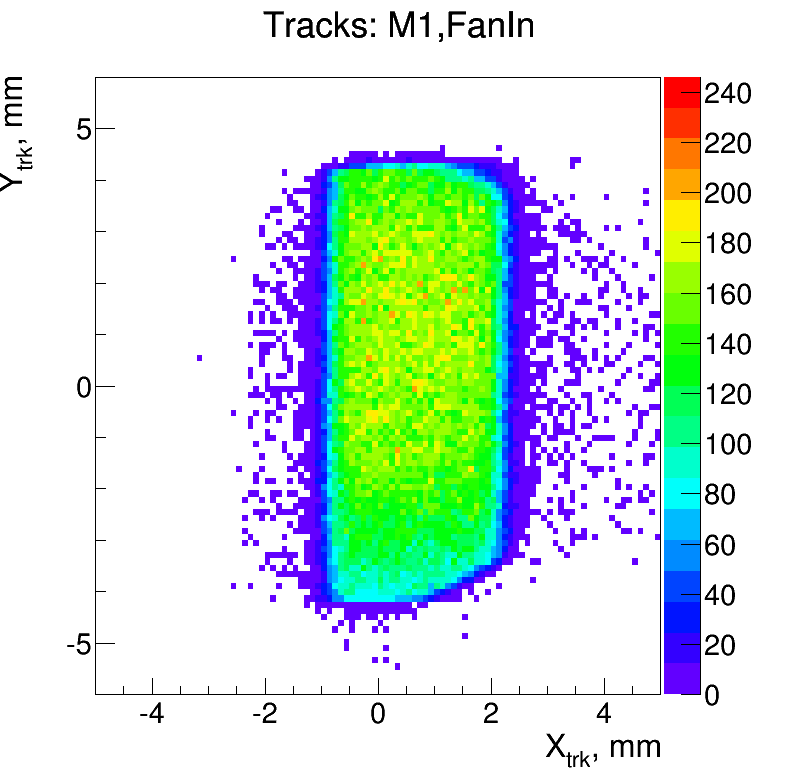
\includegraphics[width=0.5\textwidth]{figs/Tracks_2D_M1_FanIn_189_15106.png} % Central region (70,10,0)
%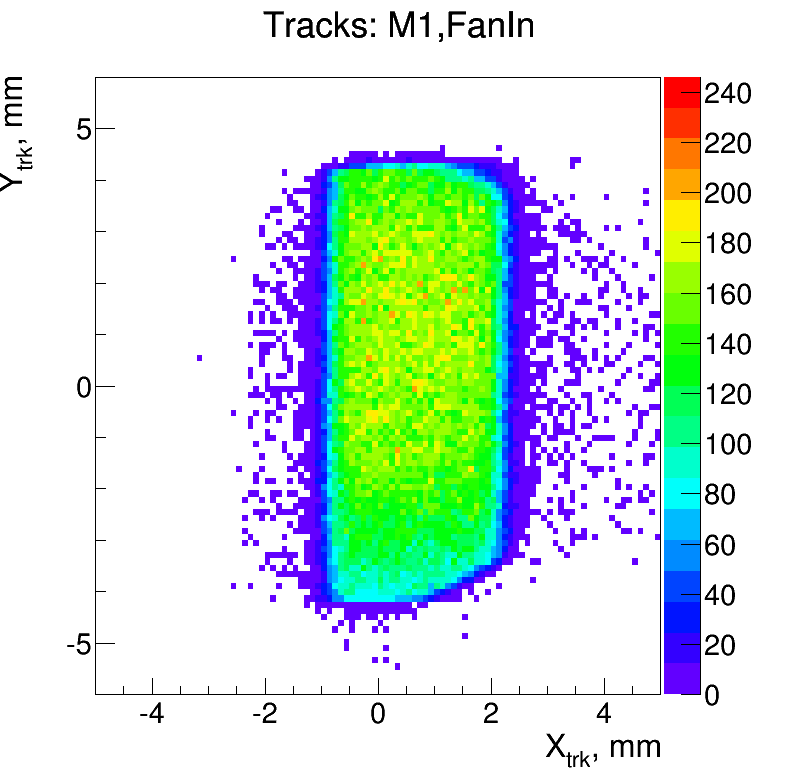
\includegraphics[width=0.5\textwidth]{figs/Tracks_2D_M1_FanIn_189_15106.png} % PA region (70,0,0)
\caption[Beam profile, as reconstructed by the telescope.]{Beam profile, as reconstructed by the telescope during the data taking for the M1 fan-in sensor (run 189).}
\label{fig:BeamProfile}
\end{figure}